\subsection{Matched scale sensitivity and source-selected reporting panels}

A further registered development supplement addresses scale and reporting gaps without enlarging the neural menu. Metadata qualification verifies that count/log2 banks share raw-source hashes, genes, target/pair identities, original development/query roles, normalizers and QC. Count models reuse the exact three random and three partner outer folds per source, with the original nested source partitions. The fixed menu retains additivity, mean residual, 24 tuned global ridge/RBF settings and 18 settings each for summed-single, pair-product and mixed kernels. The simple reference is source-selected, and neither historical evaluator nor calibration outcomes are accessed \citep{opalpanel2026}.

\begin{center}\small\begin{tabular}{lrrrr}\toprule

Count-scale track & Simple MSE & Pair MSE & Mixed MSE & Pair / mixed gain\\\midrule

norman random & 1.099782 & 1.054091 & 0.998685 & 4.15 / 9.19\%\\

norman partner & 1.846124 & 1.676695 & 1.704124 & 9.18 / 7.69\%\\

wessels random & 0.187987 & 0.198708 & 0.195647 & -5.70 / -4.07\%\\

wessels partner & 0.242347 & 0.269093 & 0.267866 & -11.04 / -10.53\%\\

\bottomrule\end{tabular}\end{center}

Norman count-scale gains are positive, unlike its log2 results, so direction is scale-sensitive. The primary gates still fail: Norman random mixed correction gains 9.19\%, with paired MSE-reduction interval $[-0.011700,0.273082]$; Norman partner pair correction gains 9.18\%, with interval $[-0.113894,0.496702]$. The other count pair/mixed intervals also span zero. Wessels count corrections worsen the reference. Raw count and log2 MSE units cannot be compared directly, and neither scale replaces the original endpoint.

Each outer source defines a strong panel by its top 10\% mean absolute pair effects. A separate low-single residual-enriched proxy ranks source residual magnitude among genes whose source single magnitudes do not exceed the median. Query pair labels cannot select either mask. All models use the same fold masks; these are diagnostic source-derived panels, not validated emergent gene sets. All nine protocols, all three panels and one/two-held-target subsets are retained.

On Norman count partner folds, the residual proxy gives pair-product and mixed gains of 12.49\% and 9.23\%, with positive conditional lower bounds. These favorable subsets do not override failed all-gene gates. The top source-selected 10\% strong genes contribute 99.17\% and 99.43\% of Norman count reference error in random and partner scoring, illustrating endpoint concentration.

\par\begin{figure}[ht]\centering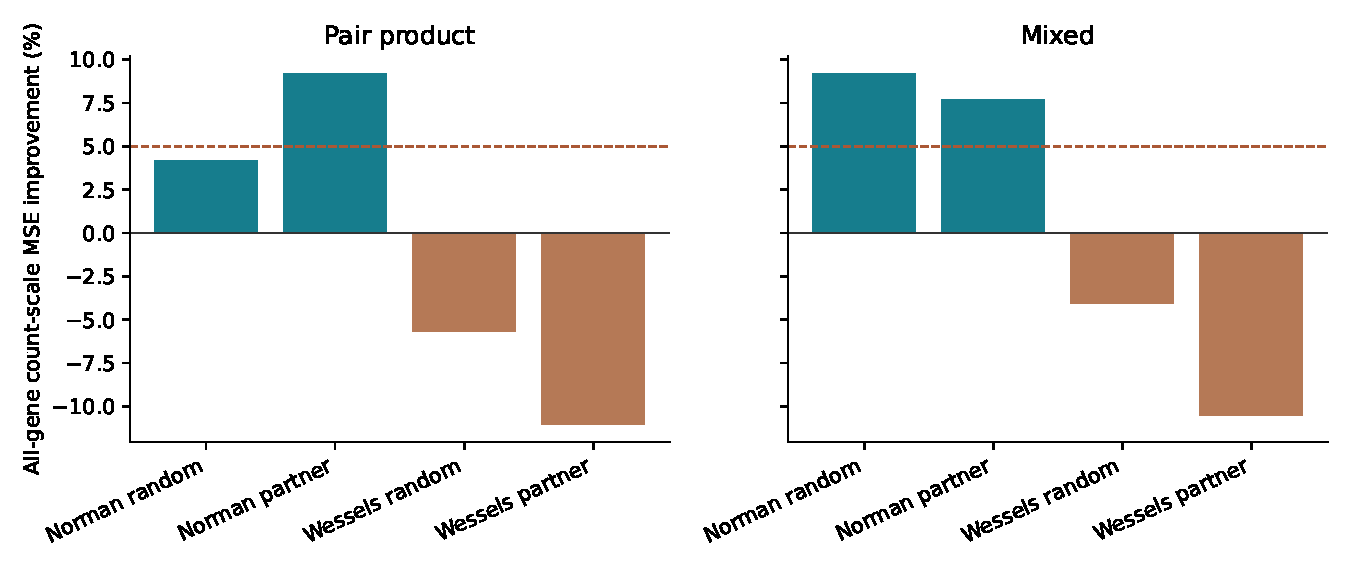
\includegraphics[width=.9\linewidth]{evidence/panel_scale_results.pdf}\caption{Count-scale point gains on Norman do not pass the paired-uncertainty gate. Wessels remains unfavorable. Full panels, intervals and target subsets are retained.}\end{figure}\par

Identity-only recovery of the original partner assignments separates 120 one-held-target and 28 two-held-target Norman occurrences, versus 58 and 11 on Wessels. These correspond to only 88 and 40 unique conditions: 60 Norman pairs and 29 Wessels pairs recur in two folds. Pairwise intersections and every coverage count are saved; repeated occurrences do not supply independent replication. Opposite technical-half diagnostics retain complete shared reference matrices and report residual MSE, direction cosine and the main/residual/cross-term identity on all panels. Frozen QC, full-reference configuration selection and source-selected masks prevent a biological-independence claim.

Count fitting takes 14.39 elapsed seconds; the complete fitting and diagnostic runner takes 37.89 seconds on one CPU thread, with 243.8 MB completion RSS, not a measured peak. No pair component advances on these primary gates. Independent cultures and sealed state/pair confirmation remain missing.
